%!TEX TS-program = xelatex 
%!TEX TS-options = -output-driver="xdvipdfmx -q -E"
%!TEX encoding = UTF-8 Unicode
%
%  my_title
%
%  Created by my_name on date.
%  Copyright (c) year. All rights reserved.
%

\documentclass[12pt]{article} 

% Definitions
\newcommand\mykeywords{color, illusion} 
\newcommand\myauthor{Mark Eli Kalderon} 
\newcommand\mytitle{Color Illusion}
\newcommand\mybib{Philosophy.bib}

% Packages
\usepackage{geometry} \geometry{a4paper} 
\usepackage{url}
\usepackage{txfonts}
\usepackage{color}
\definecolor{gray}{rgb}{0.459,0.438,0.471}
% \usepackage{setspace}
% \doublespace % Uncomment for doublespacing if necessary
\usepackage{epigraph} % optional

% XeTeX
\usepackage[cm-default]{fontspec}
\usepackage{xltxtra,xunicode}
\defaultfontfeatures{Scale=MatchLowercase,Mapping=tex-text}
\setmainfont{Palatino}
\setsansfont{Gill Sans}
\setmonofont{Inconsolata}

% Section Formatting
\usepackage[]{titlesec}
\titleformat{\section}[hang]{\fontsize{14}{14}\scshape}{\S{\thesection}}{.5em}{}{}
\titleformat{\subsection}[hang]{\fontsize{12}{12}\scshape}{\S{\thesubsection}}{.5em}{}{}
\titleformat{\subsubsection}[hang]{\fontsize{12}{12}\scshape}{\S{\thesubsubsection}}{.5em}{}{}

% Headers and Footers
\usepackage{fancyhdr}
\pagestyle{fancy}
\pagenumbering{arabic}
\lhead{\thepage}
\chead{}
\rhead{\itshape{\nouppercase{\leftmark}}}

% TODO List
\usepackage{color}
\usepackage{index} % use index package to create indices
\newindex{todo}{tod}{tnd}{TODO List} % start todo list
\newindex{fixme}{fix}{fnd}{FIXME List} % start fixme list
\newcommand{\todo}[1]{\textcolor{blue}{TODO: #1}\index[todo]{#1}} % macro for todo entries
\newcommand{\fixme}[1]{\textcolor{red}{FIXME: #1}\index[fixme]{#1}} % macro for fixme entries

% Bibliography
\usepackage[round]{natbib} 

% Title Information
\title{\mytitle} % For thanks comment this line and uncomment the line below
%\title{\mytitle\thanks{}}% 
\author{\myauthor} 
% \date{} % Leave blank for no date, comment out for most recent date

% PDF Stuff
\usepackage[plainpages=false, pdfpagelabels, bookmarksnumbered, backref, pdftitle={\mytitle}, pagebackref, pdfauthor={\myauthor}, pdfkeywords={\mykeywords}, xetex, dvipdfmx, colorlinks=true, citecolor=gray, linkcolor=gray, urlcolor=gray]{hyperref} 



%%% BEGIN DOCUMENT
\begin{document}

% Title Page
\maketitle
% \begin{abstract} % optional
% \end{abstract} 
\vskip 2em \hrule height 0.4pt \vskip 2em
% \epigraph{text of epigraph}{\textsc{author of epigraph}} % optional; make sure to uncomment \usepackage{epigraph}

% Layout Settings
\setlength{\parindent}{1em}

% Main Content

\section{Introduction} % (fold)
\label{sec:introduction}

I have lost my grip on what a color illusion is meant to be. Perhaps I have simply lost my grip---not an alternative to be ruled out in advance of inquiry. However, I believe that there is an alternative explanation. I have come to suspect that there is nothing answering to the philosopher's conception of illusion. That's not to say that there are no color experiences that might, with propriety, be described as illusory. There is a familiar genre of books illustrating optical illusions, many essentially involving chromatic phenomena. No charge of false advertising is leveled here. It is only a distinctively \emph{philosophical} conception of illusion whose claims are exaggerated. Or so I have, lately, come to suspect.

% section introduction (end)

\section{Benham's Disk} % (fold)
\label{sec:benham_s_disk}

Let's begin by considering an example of a color illusion often cited by philosophers---Benaham's disk.

In 1894, an English toymaker, Charles Benham, devised a top adorned with a black and white pattern (see Figure~\ref{fig:benham}). Sold through Messrs. Newton and Co., an announcement of the ``Artifical Spectrum Top'' was published in \emph{Nature}:
\begin{quote}
	The top consists of a disc, one half of which is black, while the other half has twelve arcs of concentric circles drawn upon it. Each arc subtends an angle of forty-five degrees. In the first quadrant there are three such concentric arcs, in the next three more, and so on ; the only difference being that the arcs are parts of circles of which the radii increase in arithmetical progression. Each quadrant thus contains a group of arcs differing in length from those of the other quadrants. The curious point is that when this disc is revolved, the impression of concentric circles of different colors is produced upon the retina. If the direction of rotation is reversed, the order of these tints is also reversed. \citep{Benham:1894kx}
\end{quote}
Specifically, if rotated clockwise, the innermost arcs form reddish rings, the next greenish rings, the next light blue rings, and the outermost arcs form violet rings. If rotated counterclockwise the pattern is reversed with the innermost arcs now forming violet rings and the outermost reddish rings. These apparent colors are puzzling. Each of the spinning arcs reflect light with the same spectral content and with equal average luminance. In advance of observing the spinning disk, then, one might reasonably expect the spinning arcs to appear as gray rings of equal brightness. The mysterious apparent colors of Benham's spinning disk are the ``subjective colors'' first described by \citep{Fechner:1838vn} (and, hence, are also sometimes described as ``Fechner-Benham colors''). The subjective colors produced by Benham's spinning disk are not completely understood; for a review of some of the color science see \citet{Campenhausen:1995yq}.

\begin{figure}[htbp]
	\centering
		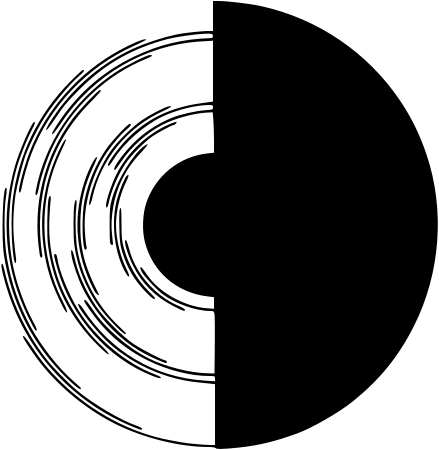
\includegraphics[scale=.5]{graphics/benhams_disk.jpg}
	\caption{Benham's Disk}
	\label{fig:benham}
\end{figure}

The subjective colors of the Benham disk are usually reckoned to be illusory. The surface of the disk is black and white. No part of the surface of the disk is reddish, or greenish, or light blue, or violet. So these apparent colors are merely apparent. In experiencing the reddish ring, we are perceiving something which is, in fact, not at all reddish. To that extent at least, the reddish appearance is \emph{illusory}. Similar reasoning holds for each of the subjective colors produced by the spinning disk.

\section{Pointillism and the Argument from Microscopes}\label{sec:pointillism_and_the_argument_from_microscopes} % (fold)

It would seem, then, that the subjective colors produced by the Benham disk are straightforward examples of color illusions as standardly conceived by philosophers. So what's the problem?

To bring the problem out, I want to compare the subjective colors produced by Benham's disks with two other chromatic phenomena. A proper understanding of these renders unsound the reasoning to the conclusion that the subjective colors produced by Benham's disk are illusory.

% section benham_s_disk (end)

\subsection{Pointillism}\label{sub:pointillism} % (fold)

Michel Eugène Chevreul, a French chemist who was serving as a director of a Parisian dye works, upon receiving complaints that the black dyes they produced looked different when used alongside blue dye, investigated the matter and discovered the phenomena of simultaneous color contrast. \citet{Chevreul:1855kx} reported his findings in his book, \emph{The Principles of Harmony and Contrast of Colours and Their Application to the Arts}, a book that influenced the work of the French paper Georges-Pierre Seurat. Fascinated by the appearance of a color being influenced by adjacent colors, Seurat eventually paints the pointillist materpiece, “Un dimanche après-midi à l'Île de la Grande Jatte” in 1884--6. Using only primary unblended pigments, including the newly invented zinc yellow, these were distributed in small dots across the surface of the canvas giving rise to the appearance, at an appropriate distance, of a differently colored scene of Parisian suburbanites relaxing by the river Seine.

Imagine, then, if you will, viewing a minimalist painting in a gallery. From your current vantage point, the surface of the painting appears a uniform if luminous green. Closer inspection is revealing, however. As you move in for a closer look, the painting is discovered to be not only minimalist, but pointillist. The luminous green appearance of the surface was achieved by painstakingly painting minute yellow and blue dots across the surface. In fact no part of the surface of the painting is green---every part of the surface is either yellow or blue. One might be tempted to conclude that the green appearance of the painting was illusory---though it would be understandable if one were to feel hesitant in giving in to temptation in this instance. If no part of the surface of the painting is green, then how could the green appearance be veridical? 

It would seem that we have here reasoning that straightforwardly parallel's the reasoning that convicted the subjective colors of being illusory. However, the reasoning in this intermediary case is fallacious as Hilbert's \citeyear[chapter 2]{Hilbert:1987jq}, discussion of Berkeley's \citeyear{Berkeley:1734fk} argument from microscopes reveals.

% subsection pointillism (end)

\subsection{The Argument from Microscopes}\label{sub:the_argument_from_microscopes} % (fold)

In arguing against the claim that ``the colors which we see exist in external bodies'', Berkeley presents the argument from microscopes:
\begin{quote}
	PHILONUS: `Apparent' colors you call them? How shall we distinguish these apparent colors from real?\\
	HYLAS: Very easily. They are to be thought apparent which appearing only at a distance, vanish upon a nearer approach.\\
	PHILONUS: And those, I suppose, are to be thought real which are discovered by the most near and exact survey.\\
	HYLAS: By a microscope, doubtless.\\
	PHILONUS: But a microscope often discovers colors in an object different from those perceived by the unassisted sight. And, in case we had microscopes mangnifying to any assigned degree, it is certain that no object whatsoever, viewed through them, would appear in the same color which it exhibits to the naked eye.\\
	HYLAS: And what will you conclude from all this? You cannot argue that there are really and naturally no colors on objects because by artificial managements they may be altered or made to vanish.\\
	PHILONUS: I think it may be evidently concluded from your own concessions that all the colors we see with our naked eyes are only apparent as those on the clouds, since they vanish upon a more close and accurate inspection which is afforded us by a microscope.
\end{quote}
The conclusion of this argument is that either the appearance of the object to the naked eye or their appearance through microscopes is illusory. But from here, all that is required to reach the claim that all color is apparent is the application of classic Pyrrhonian reasoning---justify which of these vantage points affords us knowledge of the true colors of external objects or give up the claim that colors inhere in external objects. For if the naked eye and the microscope each have equal claim to affording us knowledge of the colors of external objects, then neither do.

\citet{Hilbert:1987jq} adapts a version of the argument from microscopes due to \citet{Marc-Wogau:1968kx}. Fresh blood looks uniformly red. When viewed under a microscope, the blood appears partly red and partly transparent. 

% subsection the_argument_from_microscopes (end)

% section pointillism_and_the_argument_from_microscopes (end)

% Bibligography
\bibliographystyle{plainnat} 
\bibliography{Philosophy.bib} 

\end{document}
